

%En el año 1973 por Julius Wess y Bruno Zumino presentan un modelo en la física de partículas el cual es conocido con el nombre de Modelo de Wess-Zumino, este es un modelo mínimo supersimétrico con solo un fermión y su súper compañero bosón. A pesar de que el modelo de Wess-Zumino no representa un modelo físico real, sirvió para fundamentar ciertos aspectos de los modelos físicos supersimétricos teorizados. 

%Entre las posibles búsquedas para descifrar la composición de la materia oscura, algunas de las más populares son entre las partículas 

El primer modelo supersimétrico compatible con el modelo estándar de la física de partículas es el \MSSM, que fue enunciado en el año 1981 por Howard Georgi y Savas Dimopoulos. El modelo postula la existencia de partículas supersimétricas en la región entre $10^2-10^3~GeV$, prediciendo su aparición en los experimentos de colisiones de partículas aceleradas. %Los científicos esperan poder demostrar mediante el \LHC~ la existencia de los super compañeros de las partículas elementales ya conocidas.

El \MSSM ~ no es la única opción posible para la supersimetría más allá del \ME, %existen extensiones supersimétricas no mínimas del Modelo Estándar, 
pero sí es la más popular dada su simplicidad, introduce el higgsino, thewino, el zino, junto con todos los squarks y sleptons (ver Fig. \ref{susy}). 
%. En principio, se puede construir cualquier \textbf{SSM} (\textbf{S}uper\textbf{S}ymmetry \textbf{M}odel), sin embargo, se deben tener en cuenta varias limitaciones al realizarlo.
La única forma inequívoca de reclamar el descubrimiento de la supersimetría es producir superpartículas en el laboratorio. Debido a que se espera que las superpartículas sean de 100 a 1000 veces más pesadas que el protón, se requiere una gran cantidad de energía para generarlas %hacer estas partículas que solo se pueden lograr 
en los aceleradores de partículas. Sin embargo, ninguna de las compañeras supersimétricas de las partículas del \ME ~ han sido observadas hasta el momento.
%El Tevatron estaba buscando activamente evidencia de la producción de partículas supersimétricas antes de que se cerrara el 30 de septiembre de 2011. La mayoría de los físicos creen que se debe descubrir la supersimetría en el LHC si es responsable de estabilizar la escala débil. 
%Hay cinco clases de partículas en las que se encuentran los supercompañeros del modelo estándar: squarks, gluinos, charginos, neutralinos y sleptons. Estas superpartículas tienen sus interacciones y desintegraciones posteriores descritas por el \MSSM ~ y cada una tiene firmas características.

%La mayoría de estos parámetros conducen a una fenomenología inaceptable, como grandes corrientes neutras que cambian de sabor o grandes momentos dipolares eléctricos para el neutrón y el electrón. Para evitar estos problemas, el MSSM toma toda la ruptura de la supersimetría suave para que sea diagonal en el espacio de sabor y para que todas las nuevas fases de violación de CP desaparezcan.

\subsubsection{Lagrangiano del modelo MSSM.}
El \MSSM ~ impone la \href{https://es.wikipedia.org/wiki/Paridad\_R}{paridad R} para explicar la estabilidad del protón agregando una ruptura de supersimetría al introducir operadores explícitos en el Lagrangiano que se le comunica mediante una dinámica desconocida, significando la presencia de 120 parámetros nuevos en el \MSSM.
%Si una teoría es invariante bajo transformaciones supersimétricas, las partículas y sus correspondientes supercompañeras deben tener masas idénticas. %Es decir, si la supersimetría no estuviera rota, deberían existir selectrones con una masa igual a me ~ 0.511 MeV, y lo mismo para los demás sleptones y squarks. Y también deberían existir los gluinos y fotinos sin masa. 
Aunque no se conoce el mecanismo de ruptura de \SUSY, este debe ser implementado de forma de que pueda proveer la solución al problema de jerarquía incluso en presencia del rompimiento de ésta. Para ello, las relaciones entre los acoplamientos adimensionales de la teoría antes del rompimiento deben mantenerse. El lagrangiano efectivo del \MSSM ~ tiene la forma:
\begin{equation}\label{lagrangianoMSSM}
\mathcal{L}_\mathbf{MSSM} = ~ \mathcal{L}_\mathbf{SUSY}+\mathcal{L}_\mathbf{soft}
\end{equation}
donde $\mathcal{L}_\mathbf{SUSY}$ contiene todas las interacciones de gauge de Yukawa preservando la supersimétrica, más información en la referencia \cite{kuroda_complete_2005}. El potencial \MSSM ~viene dado por la expresión:
\begin{equation}\label{potencialMSSM}
W_\mathbf{MSSM} = Q_L Y_U H_2 U_R + Q_L Y_D H_1 D_R + L_L Y_E H_1 E_R + \mu H_2 H_1 
\end{equation}
la definición de sus términos se encuentra en la referencia \cite{kuroda_complete_2005}.
El lagrangiano que rompe \SUSY, $\mathcal{L}_\mathbf{soft}$, no está completamente determinado y su forma explícita así como el conjunto de parámetros involucrados dependen del mecanismo particular de ruptura de \SUSY ~implementado, siempre manteniéndose invariante frente $\mathbf{SU(3)_C} \otimes \mathbf{SU(2)_L} \otimes \mathbf{U(1)_Y}$. Los términos $\mathbf{soft}$ proveen exitosamente de las masas de las partículas supersimétricas, a fin de que sean más pesadas que sus correspondientes compañeras del \ME, y la ruptura espontánea de la simetría electrodébil requerida a bajas energías es necesaria para explicar la masa de las partículas.

%Debido a que la diferencia de masas entre las partículas conocidas del \ME ~y sus supercompañeras las masas de las partículas supersimétricas no pueden ser demasiado grandes, sino se perdería la solución al problema de jerarquía, pero por otro lado, también existe una razón por la cual las partículas supersimétricas deben ser lo suficientemente pesadas para no haber sido descubiertas hasta ahora. Todas las partículas del \MSSM ~que han sido observadas tienen algo en común: deberían no tener masa en ausencia del rompimiento de la simetría electrodébil. %En particular, las masas de los bosones $W^\pm$, $Z^0$, los quarks y leptones son iguales al producto de constantes de acoplamiento adimensionales por $<H> 174 GeV, mientras que el fotón y el gluón necesitan ser no masivos por la invariancia de gauge electromagnética y de QCD. Por el contrario, todas las partículas del MSSM no descubiertas tienen la propiedad contraria. 
%Además cada partícula del \MSSM ~ puede tener un término de masa en el lagrangiano en ausencia del rompimiento de la simetría electrodébil.

En un tratamiento fenomenológico completo todos los parámetros del \MSSM~ deberían dejarse libres y determinarse a partir de los datos observados, y luego de que los parámetros hayan sido medidos, de ahí se podría intentar extraer información de la física subyacente que está asociada con escalas de energía mayores a la de los experimentos. Sin embargo, realizar predicciones y análisis fenomenológicos con esta cantidad de parámetros no es posible, por lo cual es necesario realizar suposiciones para reducir los grados de libertad. Es debido a este motivo que no existe una definición precisa del \MSSM .%~y es importante conocer cuales son las suposiciones que se han hecho cuando se realiza un determinado análisis.

%\subsubsection{Insuficiencias del modelo MSSM.}
Hay además problemas con la propia teoría \MSSM, la mayoría de ellos resultado de la interpretación de los parámetros que lo componen. Por ejemplo, el parámetro de masa del Higgsino $\mu$ (último término en el superpotencial de la ec. \ref{potencialMSSM}) debe tener %el mismo orden de magnitud que la escala de electroválvula, 
muchos órdenes de magnitud menores a la escala de Planck, esta cuestión es llamada problema $\mu$. Mas aún, los términos de ruptura de la supersimetría también deben ser del mismo orden de magnitud que la escala electrodébil. Los términos adicionales en el lagrangiano del \MSSM ~ deben ser invariantes de \textbf{CP}, sin embargo hasta el momento ninguna violación de \textbf{CP} fuera del \ME ~ ha sido predicha, por lo que sus fases de violación \textbf{CP} deben ser pequeñas.

%\item[-] Universalidad de sabores de masas suaves y términos A: dado que hasta ahora no se ha descubierto una mezcla de sabores adicional a la predicha por el modelo estándar, los coeficientes de los términos adicionales en el \MSSM Lagrangiano deben ser, al menos aproximadamente, invariantes de sabores.
%\item[-] 

\subsubsection{Más allá del modelo MSSM.}
El \textbf{N}\MSSM~(\textbf{N}ext-to-\textbf{M}inimal \textbf{S}upersymmetric \textbf{S}tandard \textbf{M}odel) es una extensión supersimétrica del Modelo Estándar que agrega un término adicional en el superpotencial de la ec. \ref{potencialMSSM} para violar la simetría Peccei–Quinn por medio de un término cúbico de auto-acoplamiento, $\mu H_2 H_1 \rightarrow \lambda S H_2 H_1 + \frac{1}{3} \kappa S^3$ \citep{cms_collaboration_search_2019-1}, de esta forma se genera dinámicamente el parámetro $\mu$ resolviendo el problema derivado del mismo. En \MSSM, el sector de Higgs está altamente restringido, al extenderlo, se amplia esta restricción y se reducen las limitantes experimentales predichas en la teoría. 

Con está extensión se incluye un supercampo adicional como vimos anteriormente y se prevé la existencia de siete bosones de Higgs, tres bosones neutros $h_{1,2,3}$ con simetría CP-par, dos bosones neutros $n_{1,2}$ con CP-impar, y un par de Higgs cargados $H^\pm$. En los modelos \textbf{N}\MSSM, dos de los tres bosones de Higgs neutros pares $h_1$ o $h_2$  pueden descomponerse en uno de los dos bosones de Higgs neutros impares de \textbf{CP} a través de $h_{1,2} \rightarrow 2n_1$, este debe satisfacer la condición $2m_{n_1} < m_{h_{1,2}}$.

%En estas topologías de señal la presencia de un bosón de Higgs $h$ similar al de \ME ~ que se desintegra a través de $h \rightarrow 2n_1$, donde $n_1$ es el neutralino ligero no oscuro. Ambos $n_1$ luego decaen vía $n_1 \rightarrow n_D + \gamma_D$, donde $n_D$ es un neutralino oscuro que no es posible detectar. 


%Alternativamente, uno podría imponer un orden de terminación lineal o cuadrática para romper la simetría de Peccei-Quinn, pero nuevamente sería necesario un parámetro dimensional. Tenga en cuenta que el superpotencial debe tener una dimensión de masa tres. Por supuesto, cualquier término superior a trilineal en los campos en el superpotencial está prohibido por el requisito de renormalizabilidad. Finalmente llegamos al superpotencial NMSSM propuesto, escrito en su forma escalar
%\subsubsection{Origen de la ruptura de \SUSY.}

Debido a que no se ha observado ninguna de las partículas supersimétricas predichas, si es que existe \SUSY, ésta debe estar rota. Para mantener la solución al problema de jerarquía, incluso en presencia del rompimiento simetría, este debe ser suave incluyendo términos $\mathbf{soft}$ al lagrangiano. Para el caso de \textbf{N}\MSSM ~ el rompimiento de \SUSY ~ es introducido explícitamente. %El rompimiento de una simetría global siempre implica un modo no masivo de Nambu-Goldstone con los mismos números cuánticos que el generador de la simetría rota. 
%En el caso de la supersimetría global, el generador es la carga fermiónica, por lo tanto la partícula de Nambu-Goldstone tiene que ser un fermión de Weyl no masivo neutro, llamado goldstino. Es claro ahora que el rompimiento espontáneo de la supersimetría requiere la extensión del MSSM. 

El rompimiento espontáneo de \SUSY ~ ocurre en un ``sector oscuro''\footnote{Proceso no observable con partículas de materia oscura} con partículas que no tienen acoplamientos directos con el %los supermultipletes quirales 
``sector visible''\footnote{Procesos observables con partículas de materia bariónica} del \textbf{N}\MSSM, sin embargo, estos dos sectores comparten algunas interacciones que son las responsables de mediar el rompimiento de la supersimetría desde el sector oscuro al visible.

En modelo \SUSY ~oscuro o \textbf{Dark-\SUSY} supone como origen de la ruptura espontánea \textbf{U(1)} (una simetría global de Peccei–Quinn) el acoplamiento débil de unos fotones oscuros $\gamma_D$ a sus homólogos del \ME ~ a través de un parámetro de mezcla cinética $\epsilon$ descrito introducido en el lagrangiano:
\begin{equation}
\mathcal{L}_\mathbf{KM}\backsim \dfrac{\epsilon}{2} F_{\mu v}^{\gamma} F^{\mu v}
\end{equation}
donde $F_{\mu v}^{\gamma} = \partial_\mu A_v^{D} -\partial_v A_\mu^D$ y $A^D$ es el campo de calibración oscuro. Si el $A_D$ es masivo, entonces las partículas \textbf{SM} adquieren una carga adicional bajo la interacción con el sector oscuro. Además, en los escenarios típicos de \textbf{Dark-\SUSY}, el mezcla cinética del parámetro $\epsilon$ está dentro del intervalo $10^{-8}-10^{-2}$ \citep{cms_collaboration_search_2019-1}. En este caso se teoriza que el neutralino más ligero $n_1$ en el sector visible de \SUSY ~ ya no es estable y puede descomponerse a través de procesos como $n_1\longrightarrow  n_D + \gamma_D$, donde $n_D$ es un fermión oscuro (neutralino oscuro) que escapa a la detección con los instrumentos existentes actuales. 

Con el desarrollo del modelo \textbf{N}\MSSM ~ y los modelos de supersimetría en el sector oscuro \textbf{Dark-SUSY}, es posible teorizar un conjunto de criterios de búsqueda destinados a minimizar los eventos de fondo sin dejar de ser independientes de los modelos utilizados. Suponiendo que $\gamma_D$ solo puede descomponerse en partículas \textbf{SM}, %la fracción de decaimiento $\gamma_D\rightarrow \mu^+\mu^-$ puede variar en %ser tan grande como 45\% esto dependencia de la masa $m_{\gamma_D}$. 
muchas líneas de investigación realizan exploraciones para los posibles decaimientos $h \rightarrow 2n_1$, donde se incluye $4\mu$ \citep{cms_collaboration_search_2016,cms_collaboration_search_2013}
, $4\tau$ %\citep{khachatryan_search_2016}
, $4\ell$ \citep{cms_collaboration_search_2018,lhcb_collaboration_search_2016}
, $4\ell/4\pi$ \citep{cms_collaboration_search_2018-1}
, $4\ell/8\ell$ \citep{atlas_collaboration_search_2016-2}
, $4b$ \citep{atlas_collaboration_search_2018-1,atlas_collaboration_search_2016-3}
, $4\gamma$ \citep{atlas_collaboration_search_2014}
, $2b/2\tau$ \citep{atlas_collaboration_search_2018-2}
, $2\mu 2\tau$ \citep{atlas_collaboration_search_2015-1}
y $6q$ \citep{cms_collaboration_search_2016-2} 
como posibles estados finales, siendo estos análisis contribuciones a un cuerpo existente de trabajo experimental en la búsqueda de nuevos bosones.

El ancho parcial %cita
para la descomposición del fotón oscuro en leptones \ME ~ se tiene una expresión dado por:
\begin{equation}\label{ancho_parcial}
\Gamma_{\gamma_D \rightarrow \bar{\ell}\ell} = \dfrac{1}{3}\alpha \epsilon^2 m_{\gamma_D} \sqrt{1- \dfrac{4m_\ell^2}{m_{\gamma_D}^2}}
\left( 1 + \dfrac{2m_\ell^2}{m_{\gamma_D}^2}\right) 
\end{equation}
donde $m_\ell$ es la masa del leptón y los diferentes modos de descomposición comienzan desde $m_{\gamma_D} > 2 m_\ell$. Además, el fotón oscuro se descompondrá en hadrones del \ME ~ para masas $m_{\gamma_D} > 2 m_\pi$, con ancho parcial dado por:
\begin{equation}\label{ancho_foton}
\Gamma_{\gamma_\mathbf{D} \rightarrow ~ \mathbf{hadrones}}= \dfrac{1}{3} \alpha \epsilon^2 m_{\gamma_D} \sqrt{1 -\dfrac{4 m_{\mu^2}}{m_{\gamma_D}^2}} \left( 1 + \dfrac{2 m_\mu^2}{m_{\gamma_D}^2}\right) R(s = m_{\gamma_D}^2)
\end{equation}
donde $R = \sigma_{e^+ e^- \rightarrow ~ \mathbf{hadrons}} / \sigma_{e^+ e^- \rightarrow \mu^+ \mu^-}$. %Los datos de la sección transversal hadrónica están disponibles en la bibliografía científica resultado de varias mediciones experimentales, resultado de estas pero solo se mide a partir de $\sqrt{s}= 0.36G ~ eV / c^2$, que está por encima del umbral $2 m_\pi = 0.28~GeV / c^2$. Por lo tanto, en la región donde $ < ~ 0.36~GeV / c^2$, usamos la sección transversal para $e^+e^- \rightarrow \pi^+\pi^-$. Finalmente, para la región donde $\sqrt{s} < 2 m_\pi$, sumamos solo los anchos parciales de leptones.
Según las ecs. (\ref{ancho_parcial}) y (\ref{ancho_foton}), las dependencias del ancho parcial de $\epsilon$ y $m_{\gamma_D}$ pueden factorizarse como $ (\Gamma_{\gamma_D}/\epsilon^2)^{-1}= f (m_{\gamma_D})$, donde $f (m_{\gamma_D})$ es solo dependiente de la masa del fotón oscuro. Los anchos parciales para los diferentes modos de decaimiento del fotón oscuro y su ancho total (todos divididos por $\epsilon^2$ para demostrar solo la dependencia de los anchos con $m_{\gamma_D}$) se muestran en la Tabla \ref{an-15-455:tb1} %y Fig. \ref{an-15-455:fig4}
. La relación de ramificación para la descomposición del fotón oscuro a un par de muones $B_{\gamma_D\rightarrow \mu\mu} = \Gamma_{\gamma_D\rightarrow \mu\mu} /\Gamma_{\gamma_D Total}$ no depende de $\epsilon$, y se muestra %en la Fig. \ref{an-15-455:fig4} 
como función de $m_{\gamma_D}$. % Esta relación de ramificación $B_{\gamma_D\rightarrow\mu\mu}$ tiene un mínimo en $m_{\gamma_D}\thicksim 0.8 ~ GeV/ c^2$, donde predomina el decaimiento del fotón oscuro en hadrones. 

\begin{table}[!ht]
  \begin{center}
    \small
    \begin{tabular}{l|c|c|c|c|c|c|c|c|c} % <-- Alignments: 1st column left, 2nd middle and 3rd right, with vertical lines in between
		\toprule
		& \multicolumn{9}{c}{$m_{\gamma_D}$ ~ $\mathbf{(GeV})$}\\
		\hline
		& 0.25 & 0.275 & 0.3 & 0.4 & 0.7 & 1 & 1.5 & 2 & 8.5\\
		\midrule
       	$\Gamma_{\gamma_D \rightarrow \mu^+\mu^-} ~ \mathbf{(MeV)}$ & 1 & 1.2 & 1.9 & 2.1 & 11.4 & 8.0 & 15.5 & 20.3 & 114.6 \\
       	\hline 
       	$f(m_{\gamma_D}) ~ \mathbf{(GeV^{-1})}$ & 952.9 & 817.2 & 538.9 & 480.2 & 87.4 & 125.1 & 64.6 & 49.2 & 8.7 \\
      	\bottomrule    
    \end{tabular}
    \caption{Ancho total y $f(m_{\gamma_D})$.}
    \label{an-15-455:tb1}
  \end{center}
\end{table}

Las expresiones para los anchos parciales permiten el cálculo del tiempo de vida del fotón oscuro:
\begin{eqnarray}
\label{an-15-455:ec6}
\tau_{\gamma_D} = \dfrac{}{\Gamma_{\gamma_D Total}} =\dfrac{1}{\Gamma_{\gamma_D \rightarrow e^+ e^-} + \Gamma_{\gamma_D \rightarrow \mu^+ \mu^-} + \Gamma_{\gamma_D \rightarrow hadrons }}
\end{eqnarray}
El tiempo de vida está directamente relacionada con el parámetro $\epsilon$ y la masa del fotón oscuro se obtiene:
\begin{eqnarray}
\label{an-15-455:ec7}
\tau_{\gamma_D}(\epsilon,m_{\gamma_D}) =\dfrac{f(m_{\gamma_D})}{\epsilon^2} 
\end{eqnarray}
Es conveniente representar el tiempo de vida $\tau_{\gamma_D}$ en unidades de distancia $c\tau_{\gamma_D}$, donde $c$ es la velocidad de la luz. %También es conveniente medir $c\tau_{\gamma_D}$ en milímetros porque la sensibilidad del análisis a esta variable es $\sigma(mm)$. 
Las restricciones sobre $\epsilon$ y la masa del fotón oscuro podrían obtenerse a partir de las restricciones sobre el tiempo de vida del fotón oscuro porque están directamente relacionadas entre sí como se ve en las expresiones anteriores.

%Figura 4: Izquierda: Ancho total considerando los diferentes modos de desintegración del fotón oscuro, normalizado por e2. Derecha: ¡Relación de ramificación para gD! mm modo de decaimiento. Las expresiones para los anchos parciales permiten el cálculo de la vida útil del fotón oscuro a través de:

\begin{figure}[!t]
    \centering
    (a)
    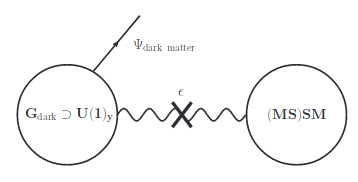
\includegraphics[width=0.55\textwidth]{Fisica_de_Particulas/imagenes/sketch_darksector.png}
    (b)
    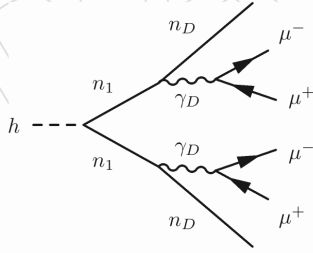
\includegraphics[width=0.35\textwidth]{Fisica_de_Particulas/imagenes/darksusy_feynman.png}
    \caption{(a) Ilustración esquemática de la conexión entre el sector oscuro y el modelo estándar, los cuales están conectados mediante un término de mezcla dinámica. (b) Diagrama de Feynman \textbf{Dark}-\SUSY ~ del proceso vía $h \rightarrow 2n_1 \rightarrow 2n_D + 2\gamma_D \rightarrow 2n_D + 4\mu$.}
    \label{fig:sketch_darksector}
\end{figure}

La descomposición del bosón ligero $n_1$ a un par de muones con carga opuesta es equivalente a $\mathcal{B}(n_1 \rightarrow 2\mu)$, con la inclusión de los modelos oscuros de \SUSY que teorizan la ruptura de una nueva simetría $U(1)_D$ dando lugar el fotón oscuro masivo $\gamma_D$, el cual es dependiente de su masa $m_{\gamma_D}$ y el parámetro de mezcla cinética. Este proceso se muestra como una posible exploración de gran interés científico. El tiempo de vida corto de la partícula $\gamma_D$ no se limita a valores pequeños ya que se espera que se mantenga estable por cierto período. Por lo que es importante acomodar la posibilidad de fotones oscuros de larga duración en las búsquedas requeridas. El diagrama de Feynman \textbf{Dark}-\SUSY ~ del proceso vía $h \rightarrow 2n_1 \rightarrow 2n_D + 2\gamma_D \rightarrow 2n_D + 4\mu$ se muestra en la Fig. \ref{fig:sketch_darksector}b. Este modelo de referencia es solo un escenario posible, y se elige como una representación única de un rango muy amplio de espacio de parámetros disponibles. %Este modelo simple del sector oscuro se puede ampliar de varias maneras; versiones más complejas involucran otros bosones oscuros de Higgs, $W$ y $Z$. También hay muchos otros procesos permitidos, como por ejemplo $pp \leftarrow h \leftarrow Z_D Z / Z_D Z_D / Z_a \leftarrow 4\mu$. En este análisis representamos los resultados de una manera que permite reinterpretaciones adicionales en el marco de otros modelos.


















